\documentclass[conference]{IEEEtran}
\usepackage[T1]{fontenc}
\usepackage{newtxtext,newtxmath}
\usepackage{amsmath}
\usepackage{graphicx}
\usepackage{booktabs}
\usepackage{multirow}
\usepackage{array}
\usepackage{siunitx}
\usepackage{xcolor}
\usepackage{tikz}
\usetikzlibrary{positioning,arrows.meta,calc,fit,backgrounds}
\usepackage[hidelinks]{hyperref}
\graphicspath{{figures/}{../figures/}}
\sisetup{group-minimum-digits=4}

% house style: no em dashes, so the abstract heading uses a colon
\makeatletter
\def\abstract{\normalfont\@IEEEabskeysecsize\bfseries\textit{\abstractname}:\ \relax\@IEEEgobbleleadPARNLSP}
\makeatother

\newcommand{\ugm}{\si{\micro\gram\per\cubic\metre}}
\newcommand{\PM}{PM\textsubscript{2.5}}
\definecolor{cres}{HTML}{2A78D6}
\definecolor{cafno}{HTML}{EB6834}
\definecolor{cgray}{HTML}{6B6B66}
\definecolor{cphys}{HTML}{1BAF7A}

% allow more floats per page so tables and figures stay near their text
\renewcommand{\topfraction}{0.9}
\renewcommand{\bottomfraction}{0.6}
\renewcommand{\textfraction}{0.08}
\renewcommand{\floatpagefraction}{0.8}
\renewcommand{\dbltopfraction}{0.9}
\renewcommand{\dblfloatpagefraction}{0.8}
\setcounter{topnumber}{3}
\setcounter{bottomnumber}{2}
\setcounter{totalnumber}{5}
\setcounter{dbltopnumber}{3}

\begin{document}

\title{Pipeline before backbone: 16-hour \PM{} forecasting over India with Fourier neural operators and convolutional-recurrent networks}

\author{\IEEEauthorblockN{Vetriselvan R, Hrishi Dongre, Pampana Sree Adithya, Ishan Goyal, Vedant Madne}
\IEEEauthorblockA{Team T024, Section A - DL Project 19: Air quality forecasting via gradient boosting and LSTM models}}

\maketitle

\begin{abstract}
We forecast \PM{} over all of India 16 hours ahead, on a $140\times124$ grid of about 25~km cells, from 10 hours of WRF-Chem simulation fields. Phase 1 forecast one Beijing station with gradient boosting. Phase 2 uses deep learning and asks how much of a forecaster's skill comes from its network and how much from the pipeline around it. Over seven development iterations we built a physics-informed pipeline: ventilation, advection and tendency channels, a log-space persistence residual, a leak-free temporal validation, a loss matched to the evaluation metric, and seed ensembles with per-hour calibration. Five networks were then trained inside this one pipeline, with decision rules fixed before each stage and 1, 2 and 5 seeds. A U-Net with a convolutional GRU over lead time (ResGRU-UNet, 7.1M parameters) beats an adaptive Fourier neural operator hybrid (AFNO V4, 7.0M) on all 25 seed pairs and at every lead hour. On 214 validation windows its five-seed mean reaches MAE 6.32~\ugm, RMSE 18.04 and $R^2$ 0.892, against 6.99, 19.45 and 0.874 for AFNO V4, 8.51, 21.48 and 0.847 for ridge regression, and 10.44, 26.46 and 0.767 for persistence: 31.8\% lower RMSE than persistence. On the held-out test set it scores 0.8914 against 0.8848. Moving the same network into the improved pipeline gained 6 to 8 times more than swapping the network. Four single-change ablations do not explain the gap between the networks; training curves show that AFNO V4 generalizes less well to unseen months. An ML + DL hybrid, a gradient-boosted correction of the ensemble forecast tested with one month left out, lowers RMSE to 17.75 but lowers the benchmark score from 0.9193 to 0.9051 in all four months, so it is reported and not adopted.
\end{abstract}

\section{Introduction}
Fine particulate matter (\PM) is the largest environmental health risk in India: air pollution was linked to an estimated 1.67 million deaths there in 2019 \cite{pandey2021}. Country-wide forecasts usually come from chemistry transport models such as WRF-Chem \cite{grell2005}, which couple weather, emissions, chemistry and transport and are expensive to run. A deep network that learns to step such a model forward from its recent fields could forecast at a small fraction of the cost.

Phase 1 \cite{phase1} forecast \PM{} six hours ahead at one Beijing station with gradient boosting, and planned deep models for Phase 2. Phase 2 moves to a larger problem: 17{,}360 grid cells, 16 lead hours, and weather fields that carry pollution across the map. Two families of deep networks suit gridded forecasting. Fourier neural operators mix the whole map at once in the frequency domain \cite{li2021fno,guibas2022afno}. Convolutional-recurrent networks pass local information step by step \cite{shi2015convlstm,ballas2016convgru}. Published comparisons between them usually change the inputs, validation, loss and post-processing along with the network, so a difference in score cannot be credited to the network alone.

Our contributions are:
\begin{itemize}
\item a physics-informed, leak-free pipeline built over seven iterations, with the reason for each move and its measured effect (Sections~\ref{sec:theory} to \ref{sec:history});
\item a controlled study of five networks inside that one pipeline, with decision rules fixed before each stage and 1, 2 and 5 seeds (Section~\ref{sec:study});
\item MAE, RMSE and $R^2$ for every model against persistence, seasonal-naive and ridge baselines, maps of where the errors fall, and the finding that model rankings depend on the metric (Section~\ref{sec:results});
\item an ML + DL hybrid, a gradient-boosted correction of the network ensemble, tested out of fold under a rule fixed before the run (Section~\ref{sec:hybrid});
\item ablations and training curves that test why the convolutional-recurrent network wins (Section~\ref{sec:ablation}).
\end{itemize}

\section{Related work}
\label{sec:related}
\textbf{Chemistry transport and emulation.} WRF-Chem runs weather and chemistry together on one grid with one transport scheme \cite{grell2005}. For particulate matter over the Indian subcontinent, lightweight deep networks were reported to beat the Aurora foundation model at short horizons \cite{kushwaha2025}. CoNOAir, a complex neural operator, is reported to beat the Fourier neural operator for carbon monoxide in Indian cities \cite{bedi2025conoair}.

\textbf{Neural operators.} The Fourier neural operator (FNO) learns maps between function spaces with convolutions in Fourier space \cite{li2021fno}. The adaptive FNO (AFNO) replaces FNO's weight per mode with a small shared MLP over blocks of channels and a soft threshold that keeps the spectrum sparse \cite{guibas2022afno}. AFNO is the backbone of the FourCastNet global weather model \cite{pathak2022fourcastnet}, and AdaptFNO adds multiscale learning for climate fields \cite{dang2025adaptfno}.

\textbf{Convolutional-recurrent forecasting.} ConvLSTM replaced the matrix products of an LSTM with convolutions for precipitation nowcasting \cite{shi2015convlstm}; TrajGRU followed \cite{shi2017trajgru}, and the convolutional GRU is the gated-recurrent version \cite{ballas2016convgru}. U-Net's skip connections pass fine detail from encoder to decoder \cite{ronneberger2015unet}, and residual learning makes deep stacks easy to train \cite{he2016}. SimVP showed that a purely convolutional encoder, translator and decoder can match recurrent models \cite{gao2022simvp}. Shortcut recurrent-convolutional U-Nets were used for weather prediction \cite{leinonen2021}.

\textbf{Training and evaluation.} We use AdamW \cite{loshchilov2019}, the one-cycle schedule \cite{smith2019}, GroupNorm \cite{wu2018}, weight averaging \cite{polyak1992} and deep ensembles \cite{lakshminarayanan2017}. SMAPE is not symmetric in additive error \cite{goodwin1999}; dependent data need blocked rather than random validation \cite{roberts2017}, and information the model would not have at forecast time inflates scores \cite{kaufman2012}. Persistence and seasonal-naive are the standard forecasts to beat \cite{hyndman2021}, and ridge regression \cite{hoerl1970} is our classical model.

\section{Data and what the exploration showed}
\label{sec:data}
The data are WRF-Chem simulation fields released by the organizers of the ANRF AISEHack 2026 challenge (Theme 2, IIT Delhi) \cite{aisehack2026}. Training covers four months of 2016, one per season (April, July, October and December; 715 or 739 hours each), on a Mercator grid of $140\times124$ cells from 7.06 to 38.00$^\circ$N and 67.79 to 97.93$^\circ$E, about 25~km apart. Each hour has 16 fields: surface \PM{} (the target), humidity, 2-m temperature, 10-m wind ($u,v$), downward shortwave radiation, boundary-layer height (PBLH), surface pressure, rain, and seven emission fields. The test set is 218 windows of 10 hours from 2017; its answers are hidden and scored by the organizers' evaluation server. Table~\ref{tab:eda} lists what the data showed and what each finding changed.

\begin{table}[!t]
\centering
\caption{What the data showed (training months) and what it changed}
\label{tab:eda}
\begin{tabular}{@{}p{0.55\columnwidth}p{0.37\columnwidth}@{}}
\toprule
Finding & What the model gets \\
\midrule
Right-skewed: December mean 59.1, median 23.7~\ugm & Work in $\log(1+y)$ \\
Lag-1 autocorrelation of $\log(1+y)$ is 0.978; the standard deviation of its change grows from 0.101 at 1 h to 0.505 at 16 h & Predict the change from persistence; weight later hours more \\
Mean 10-m wind 4.24~m/s: \PM{} moves about 10 cells in 16 h & Advection channel; a local receptive field suffices \\
Strong daily cycle (correlation 0.571 at 24 h); test windows carry no clock & Estimated hour; diurnal anomaly \\
Hotspots over the Indo-Gangetic Plain and the eastern coal belt; monthly means 15.4 (July) to 59.1 (December) & Per-cell normalization; static climatology \\
Episodes are about 2\% of cell-hours and are defined on the truth & Episode-weighted loss; calibration \\
Emission fields are tiny ($10^{-8}$ to $10^{-7}$) & Not used \\
\bottomrule
\end{tabular}
\end{table}

\textbf{Episodes.} For each cell, a robust STL decomposition \cite{cleveland1990} with a 24-hour period splits the month into trend, daily cycle and residual. An hour is an episode when its residual exceeds three standard deviations of that cell's residuals and its value exceeds 1~\ugm.

\section{Setup and fair testing}
\label{sec:setup}
\subsection{Task}
Given the fields $\mathbf{X}_{t-9:t}$ of the last 10 hours, one network forecasts all 16 hours at once,
\begin{equation}
\hat{\mathbf{y}}_{t+h} = f_\theta(\mathbf{X}_{t-9:t})_h, \qquad h = 1,\dots,16,
\end{equation}
where each $\hat{\mathbf{y}}_{t+h}$ is a $140\times124$ map of \PM{} in \ugm. This is regression.

\subsection{Validation without leaks}
A window spans 26 hours (10 in, 16 out). Two windows whose starts differ by $s$ hours share $(26-s)/26$ of their hours, so with a random split almost every validation window has a training neighbour that shares 24 or 25 of its hours, including most of its answers \cite{roberts2017}. Our early iterations used such a split and their validation scores were inflated. We hold out the last 18\% of every month, leave a 12-hour gap before it, and validate on 214 windows (stride 2); training uses the 2{,}257 earlier windows. Every model is scored on the same 214 windows.

\subsection{Scores}
With $\mathrm{SMAPE}(p,y)=|p-y|/\bigl(\tfrac12(|p|+|y|)\bigr)$, let $G$ be the mean SMAPE over all cells and hours, $E$ its mean over episode cells, and $\rho$ the Pearson correlation of forecast and truth over episode cells, per hour and averaged. The benchmark score is
\begin{equation}
S = w_1\bigl(1-\tfrac{G}{2}\bigr) + w_2\,\tfrac{1+\rho}{2} + w_3\bigl(1-\tfrac{E}{2}\bigr).
\end{equation}
The weights are not disclosed, so on validation we use $w_i=1/3$. $S$ is a composite of relative error and correlation, not an accuracy. With errors $e_i=\hat{y}_i-y_i$ over all $n = 5.9\times10^7$ validation values,
\begin{gather}
\mathrm{MAE}=\tfrac1n\textstyle\sum_i|e_i|, \qquad \mathrm{RMSE}=\sqrt{\tfrac1n\textstyle\sum_i e_i^2}, \\
R^2 = 1-\frac{\sum_i e_i^2}{\sum_i (y_i-\bar{y})^2}, \qquad \text{skill} = 1-\frac{\mathrm{RMSE}}{\mathrm{RMSE}_{\text{persistence}}},
\end{gather}
as in Phase 1 \cite{phase1}. MAE, RMSE and $R^2$ exist only for validation, because the test answers are hidden; the test set gives only $S$. Note that $\rho^2$ is not $R^2$: $\rho$ ignores bias and scale.

\subsection{Decision rules and checks}
Before each stage of the study we wrote down how the result would be read. A network is called better only if it leads by more than 0.003 on validation and also scores higher on the test set; a smaller gap is a tie, and disagreement is inconclusive. Every training run and every main analysis was first run on synthetic data on a CPU, and every analysis recomputes the earlier numbers it depends on: for example, the regression metrics recompute each model's validation score and match its logged value within $10^{-4}$.

\section{Theory behind the design}
\label{sec:theory}
\textbf{Why log space.} For $p,y>0$ write $u=\log(p/y)$. Then
\begin{equation}
\mathrm{SMAPE}(p,y) = \frac{|p-y|}{(p+y)/2} = 2\,\bigl|\tanh(u/2)\bigr|,
\end{equation}
since $(p-y)/(p+y)=(e^u-1)/(e^u+1)$. SMAPE is therefore symmetric in the log ratio: twice too high and half too low cost the same, 0.667. Because SMAPE grows with $|u|$, the median minimizes the expected global SMAPE whenever $\log y$ is symmetric and unimodal around it. A network that predicts in $\log(1+y)$ works in the geometry the metric uses, and the log also tames the heavy right tail.

\textbf{Why a persistence residual.} Every network outputs a change $\Delta_h$ added to the last observed hour,
\begin{equation}
\hat{y}_{t+h} = \exp\bigl(\log(1+y_t) + \Delta_h\bigr) - 1,
\end{equation}
with the last layer set to zero at the start \cite{he2016}. An untrained network is therefore exactly persistence, which already scores 0.8515 on validation, and training only has to learn the departure from it.

\textbf{Why the episode terms reward upward shifts.} Episode cells are picked from the truth: where $y$ turned out high against its usual level. On those cells the truth is on average 50\% above persistence (mean $\log(y/\text{persistence})=+0.406$, against $-0.012$ over all cells). A forecast that cannot see the future noise therefore tends to score better on $E$ when it is shifted up; for persistence, the scale that maximizes the score rises with lead time from 1.00 to 1.30. Pearson $\rho$ does not change when a forecast is scaled, so a per-hour factor $c_h\ge1$ moves only the SMAPE terms. This is the basis of the calibration in Section~\ref{sec:training}.

\textbf{How far must a forecast see.} At the mean wind of 4.24~m/s, \PM{} travels 244~km in 16 hours: 9.8 cells, or 11.5 cells at the RMS wind. Table~\ref{tab:cost} compares the reach and cost of the main operators for $N$ cells, $d$ channels and kernel size $k$. A $3\times3$ convolution reaches one more cell per layer: ResGRU-UNet's encoder alone reaches about 14 cells, and each ConvGRU step at $18\times16$ adds about 8 more, so it covers the needed radius. AFNO mixes the whole map in every block, at a cost close to linear in $N$, but transport over 16 hours does not need global reach.

\begin{table}[!t]
\centering
\caption{Cost and reach per layer ($N$ cells, $d$ channels, $b$ blocks, $N_f$ Fourier modes)}
\label{tab:cost}
\setlength{\tabcolsep}{4pt}
\begin{tabular}{@{}lll@{}}
\toprule
Operator & Cost (multiply-adds) & Reach per layer \\
\midrule
Self-attention & $2N^2d$ & whole map \\
AFNO block & $\approx 2.5\,dN\log_2N + 8N_fd^2/b$ & whole map \\
Convolution $k\times k$ & $Nk^2d_{\text{in}}d_{\text{out}}$ & $+(k-1)/2$ cells \\
ConvLSTM step & $Nk^2(d_x+d_h)\,4d_h$ & $+(k-1)/2$ cells \\
\bottomrule
\end{tabular}
\end{table}

\section{Physics-informed inputs}
\label{sec:physics}
Surface \PM{} changes through emission, transport, vertical mixing, chemistry and deposition. Three of these leave a mark in the available fields, and we compute each one as an input instead of leaving the network to find it. Table~\ref{tab:features} lists the 20 channels.

\textbf{Vertical mixing.} The boundary layer dilutes surface pollution in proportion to its depth and the wind that flushes it. Their product, the ventilation coefficient, measures how easily the air clears; its long decline over Indian cities goes with rising pollution potential \cite{iyer2013}. We add
\begin{equation}
V = \log\bigl(1+\mathrm{PBLH}\cdot\|\mathbf{u}_{10}\|\bigr)
\end{equation}
and the wind speed $\|\mathbf{u}_{10}\|$. Low $V$ is stagnant air, where episodes build.

\textbf{Transport.} To first order a tracer follows $\partial_t C = -\mathbf{u}\cdot\nabla C$, so we add the advection of the log concentration,
\begin{equation}
A = -\bigl(u\,\partial_x + v\,\partial_y\bigr)\log(1+C),
\end{equation}
from centred differences. Earlier models used the same physics in other forms: ConvLSTM shifted the \PM{} map along the wind (a semi-Lagrangian step \cite{staniforth1991}), and FMG-WACLU added wind direction and divergence, since converging wind ($\nabla\cdot\mathbf{u}<0$) traps pollution.

\textbf{Time.} A window-local tendency $\Delta_t\log(1+C)$, divided by its per-cell spread, separates building from clearing episodes. The test windows carry no clock, so each window's start hour is estimated by matching its mean sunlight and temperature to hourly templates from training; this is right within one hour for 97.7\% of validation windows, and validation uses the estimate exactly as the test does. The hour enters as $(\sin,\cos)$, with the departure of $\log(1+C)$ from the cell's usual value at that hour, which mirrors the STL residual that defines an episode.

\textbf{Normalization.} \PM{} and rain are log-transformed; every channel is standardized per cell with training-period statistics, with a floor on the standard deviation and clipping at $\pm10$.

\begin{table}[!t]
\centering
\caption{The 20 input channels in four groups}
\label{tab:features}
\begin{tabular}{@{}lrp{0.6\columnwidth}@{}}
\toprule
Group & $n$ & Channels \\
\midrule
Weather & 9 & $\log(1+\text{\PM})$, humidity, temperature, $u_{10}$, $v_{10}$, PBLH, pressure, shortwave radiation, $\log(1+\text{rain})$ \\
Physics & 3 & wind speed, ventilation $V$, advection $A$ \\
Time & 4 & tendency, hour $\sin$ and $\cos$, diurnal anomaly \\
Static & 4 & latitude, longitude, cell \PM{} climatology, cell STL residual spread \\
\bottomrule
\end{tabular}
\end{table}

\section{Architectures}
\label{sec:arch}
Table~\ref{tab:models} lists the five networks. All read the same 20 channels and all output the residual of Section~\ref{sec:theory}. Each was ported from its original code; with the original input width and the same weights, each port reproduces the original output exactly (for ConvLSTM, with its season input, which these data lack, set to identity). A bug in the original patch AFNO, which dropped the imaginary half of every filtered spectrum, was fixed. Fig.~\ref{fig:arch} shows the two finalists.

\begin{table}[!t]
\centering
\caption{The five networks (study versions, 20 input channels)}
\label{tab:models}
\setlength{\tabcolsep}{3pt}
\begin{tabular}{@{}lrp{0.58\columnwidth}@{}}
\toprule
Network & Params & Design and inductive bias \\
\midrule
ResGRU-UNet & 7.12M & all 10 hours stacked as 200 channels; conv U-Net; ConvGRU unrolled over the 16 lead hours \\
AFNO V4 & 6.98M & per-hour conv encoder; AFNO blocks at two scales; temporal translator; U-Net decoder \\
FMG-WACLU & 3.45M & ConvLSTM U-Net with wind physics and a gate from forecast weather \\
patch AFNO & 5.71M & $4\times4$ patches, AFNO blocks, linear unpatchify \\
ConvLSTM & 19.0M & ConvLSTM over the inputs, spectral block, wind-shift advection \\
\bottomrule
\end{tabular}
\end{table}

\begin{figure*}[!t]
\centering
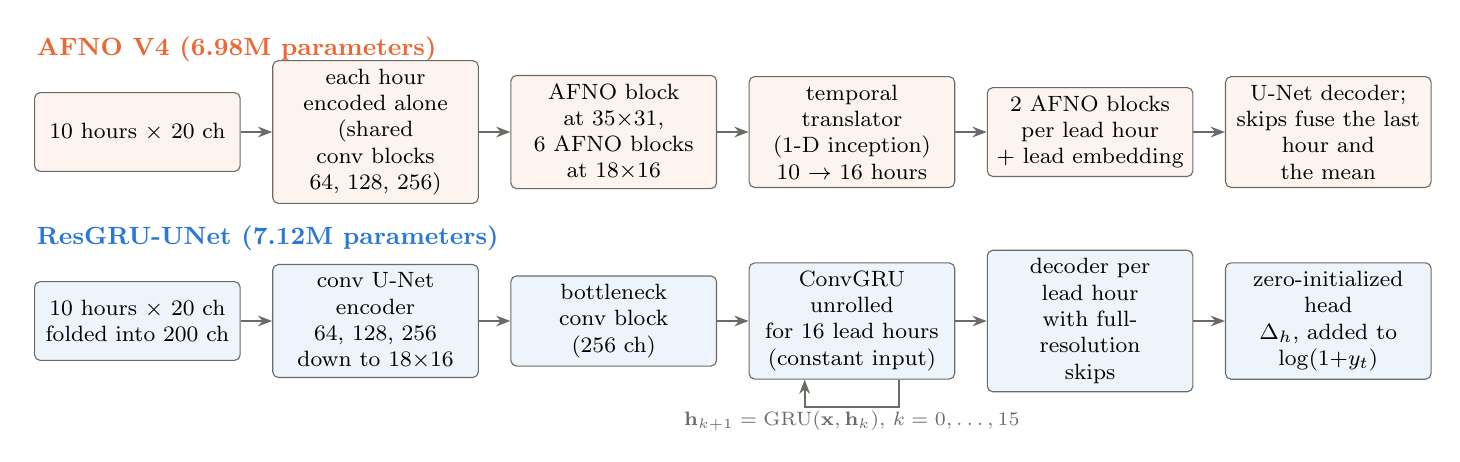
\begin{tikzpicture}[font=\footnotesize, node distance=4mm,
  b/.style={draw=cgray, rounded corners=2pt, align=center, minimum height=10mm, inner sep=3pt, text width=24mm},
  arr/.style={-{Stealth[length=1.8mm]}, cgray, thick}]
\node[font=\small\bfseries, text=cafno, anchor=west] at (-1.4,1.05) {AFNO V4 (6.98M parameters)};
\node[b, fill=cafno!8] (a0) at (0,0) {10 hours $\times$ 20 ch};
\node[b, fill=cafno!8, right=of a0] (a1) {each hour encoded alone\\ (shared conv blocks\\ 64, 128, 256)};
\node[b, fill=cafno!8, right=of a1] (a2) {AFNO block at $35{\times}31$,\\ 6 AFNO blocks\\ at $18{\times}16$};
\node[b, fill=cafno!8, right=of a2] (a3) {temporal translator\\ (1-D inception)\\ 10 $\to$ 16 hours};
\node[b, fill=cafno!8, right=of a3] (a4) {2 AFNO blocks\\ per lead hour\\ + lead embedding};
\node[b, fill=cafno!8, right=of a4] (a5) {U-Net decoder;\\ skips fuse the last\\ hour and the mean};
\foreach \i/\j in {a0/a1,a1/a2,a2/a3,a3/a4,a4/a5} \draw[arr] (\i)--(\j);
\node[font=\small\bfseries, text=cres, anchor=west] at (-1.4,-1.35) {ResGRU-UNet (7.12M parameters)};
\node[b, fill=cres!8] (r0) at (0,-2.4) {10 hours $\times$ 20 ch\\ folded into 200 ch};
\node[b, fill=cres!8, right=of r0] (r1) {conv U-Net encoder\\ 64, 128, 256\\ down to $18{\times}16$};
\node[b, fill=cres!8, right=of r1] (r2) {bottleneck\\ conv block\\ (256 ch)};
\node[b, fill=cres!8, right=of r2] (r3) {ConvGRU unrolled\\ for 16 lead hours\\ (constant input)};
\node[b, fill=cres!8, right=of r3] (r4) {decoder per lead hour\\ with full-resolution\\ skips};
\node[b, fill=cres!8, right=of r4] (r5) {zero-initialized head\\ $\Delta_h$, added to\\ $\log(1{+}y_t)$};
\foreach \i/\j in {r0/r1,r1/r2,r2/r3,r3/r4,r4/r5} \draw[arr] (\i)--(\j);
\draw[arr] ([xshift=6mm]r3.south) -- ++(0,-3.5mm) -- ([xshift=-6mm,yshift=-3.5mm]r3.south) -- ([xshift=-6mm]r3.south);
\node[below, font=\scriptsize, text=cgray, inner sep=1pt] at ([yshift=-3.6mm]r3.south) {$\mathbf{h}_{k+1}=\mathrm{GRU}(\mathbf{x},\mathbf{h}_k)$, $k=0,\dots,15$};
\end{tikzpicture}
\caption{The two finalists. AFNO V4 encodes each input hour separately and mixes the sequence in a coarse spectral bottleneck; its skip connections keep only the last hour and the mean of the 10 hours. ResGRU-UNet stacks all hours as channels in its first convolution and steps a convolutional GRU through the 16 lead hours. Both output the change $\Delta_h$ from persistence.}
\label{fig:arch}
\end{figure*}

\textbf{AFNO block.} Let $\hat{\mathbf{z}}=\mathrm{FFT}_2(\mathbf{z})$ be the orthonormal 2-D real Fourier transform of a feature map whose channels are split into $b=8$ blocks. At every Fourier mode, each block passes the same small complex MLP, then a soft threshold $S_\lambda$:
\begin{equation}
\mathcal{A}(\mathbf{z}) = \mathbf{z} + \mathrm{FFT}_2^{-1}\Bigl(S_\lambda\bigl(W_2\,\mathrm{ReLU}(W_1\hat{\mathbf{z}}+\mathbf{b}_1)+\mathbf{b}_2\bigr)\Bigr),
\end{equation}
with $\lambda=0.01$ and the ReLU applied to the real and imaginary parts separately \cite{guibas2022afno}. An AFNO block computes $\mathbf{x}\leftarrow\mathbf{x}+\mathcal{A}(\mathrm{GN}(\mathbf{x}))$, then $\mathbf{x}\leftarrow\mathbf{x}+\mathrm{MLP}(\mathrm{GN}(\mathbf{x}))$ with a $1\times1$ MLP of width $2d$ and GroupNorm GN. Every block sees the whole map, and the FFT treats opposite edges as neighbours.

\textbf{ConvGRU.} The bottleneck feature $\mathbf{x}$ is fed at every lead hour $k$ and a hidden state $\mathbf{h}_k$ is updated with $3\times3$ convolutions $*$ \cite{ballas2016convgru}:
\begin{align}
[\mathbf{r},\mathbf{u}] &= \sigma\bigl(W_g * [\mathbf{x},\mathbf{h}_k]\bigr), \\
\tilde{\mathbf{h}} &= \tanh\bigl(W_c * [\mathbf{x},\mathbf{r}\odot\mathbf{h}_k]\bigr), \\
\mathbf{h}_{k+1} &= (1-\mathbf{u})\odot\mathbf{h}_k + \mathbf{u}\odot\tilde{\mathbf{h}},
\end{align}
starting from $\mathbf{h}_0=\mathbf{x}$, with GroupNorm inside each gate. The recurrence runs over lead time, not over the input hours: the inputs enter once, through the stacked channels, and each $\mathbf{h}_{k}$ is decoded with the encoder's skips into the change for lead hour $k$.

\textbf{Other networks.} FMG-WACLU is a ConvLSTM U-Net that adds wind speed, direction and divergence and gates its features with weather rolled forward by a second ConvLSTM. ConvLSTM reads the 10 input hours recurrently at full resolution, adds an FNO-style spectral block, and shifts the \PM{} map along the wind. Patch AFNO cuts the map into $4\times4$ patches, mixes them with AFNO blocks and maps each patch back with one linear layer.

\section{Training and regularization}
\label{sec:training}
\textbf{Loss.} Training minimizes a loss matched to the score,
\begin{equation}
\mathcal{L} = 0.40\,\mathcal{H}_{\log} + 0.25\,G + 0.15\,E + 0.20\,(1-\rho),
\end{equation}
where $\mathcal{H}_{\log}$ is the Huber loss on $\log(1+y)$ with episode cells weighted by 6. Lead hours are weighted linearly from 0.7 to 1.3 in $\mathcal{H}_{\log}$ and $G$, because errors grow with lead time while the score weights all hours equally. In the loss, $G$ and $E$ add 0.1 to the SMAPE denominator for stable gradients.

\textbf{Optimization.} AdamW \cite{loshchilov2019} with learning rate $2.5\times10^{-4}$ and weight decay $10^{-4}$, a one-cycle schedule \cite{smith2019}, 16 epochs, effective batch 4, mixed precision and gradient clipping at 1.0. One run takes about 51 minutes (ResGRU-UNet) or 90 minutes (AFNO V4) on one NVIDIA T4.

\textbf{Regularization.} The networks have 3 to 19 million parameters but see only 2{,}257 training windows from four months, so we use several controls, each for a stated reason:
\begin{itemize}
\item channel dropout ($p=0.1$) in every convolution block of ResGRU-UNet and AFNO V4 and in AFNO V4's MLPs; ConvLSTM uses dropout 0.25 and stochastic depth 0.15;
\item decoupled weight decay $10^{-4}$;
\item an exponential moving average of the weights (decay 0.999) \cite{polyak1992}, which is the model we evaluate;
\item selection of the best epoch by the validation score, which acts as early stopping;
\item gradient clipping, per-cell standardization with floors, and input clipping, against rare extreme values;
\item averaging seeds \cite{lakshminarayanan2017}, which removes part of the variance between runs.
\end{itemize}
Even so, the training curves in Section~\ref{sec:ablation} show AFNO V4 fitting the training months more closely than ResGRU-UNet and doing worse on the held-out months.

\textbf{Calibration.} After ensembling, each lead hour is multiplied by a factor $c_h$ fitted on validation from a 21-point grid in $[0.90,1.10]$ to maximize the two SMAPE terms. The fitted factors rise with lead time from 1.00 to 1.08--1.10, as the episode argument in Section~\ref{sec:theory} predicts. We also fit them on three months and test on the fourth (leave one month out), to report calibration without using the scored month.

\section{How the pipeline was developed}
\label{sec:history}
The pipeline of Sections~\ref{sec:setup} to \ref{sec:training} was not designed in one go. It grew over seven iterations, each started by a problem that the previous one exposed; the controlled study is iteration 8. Table~\ref{tab:iterations} lists each move and its reason, and Fig.~\ref{fig:evolution} shows the test score. Iterations 1 to 4 were chosen on a random validation split, which leaked (Section~\ref{sec:setup}), and on feedback from part of the test set, so only their test scores are comparable.

\begin{table*}[!t]
\centering
\caption{Development iterations: what changed, why, and the held-out test score}
\label{tab:iterations}
\begin{tabular}{@{}c>{\raggedright\arraybackslash}p{0.39\textwidth}>{\raggedright\arraybackslash}p{0.41\textwidth}r@{}}
\toprule
\# & Change & Why & Test \\
\midrule
1 & AFNO on $4\times4$ patches, random split & first model: spectral mixing as in global weather models \cite{pathak2022fourcastnet} & 0.8218 \\
2 & U-Net + ConvGRU; output added to the last hour; log Huber loss & AFNO stalled below 0.83; keep local detail and sharp peaks & 0.8506 \\
3 & fine-tunes: 20 times the loss on missed episode peaks, then pinball loss ($q=0.75$) & peaks were under-predicted & 0.8594 \\
4 & blends with models trained at $q=0.85$ and $0.90$ & a stronger upward shift & 0.8648 \\
5 & temporal hold-out; AFNO with a SimVP translator, blended with ResGRU-UNet & the random split leaked & 0.8561 \\
6 & V3: official STL episodes, exact score for selection, 12-h gap, hour estimation & validation must measure what the test measures & 0.8609 \\
7 & V4: physics channels, multiscale block, lead-hour weights, 2 seeds, calibration & V3's diagnosis: long-lead errors and a global-episode trade-off & 0.8833 \\
8 & ResGRU-UNet in the V4 pipeline, 5 seeds, calibration & compare networks with the pipeline fixed & \textbf{0.8914} \\
\bottomrule
\end{tabular}
\end{table*}

\begin{figure*}[!t]
\centering
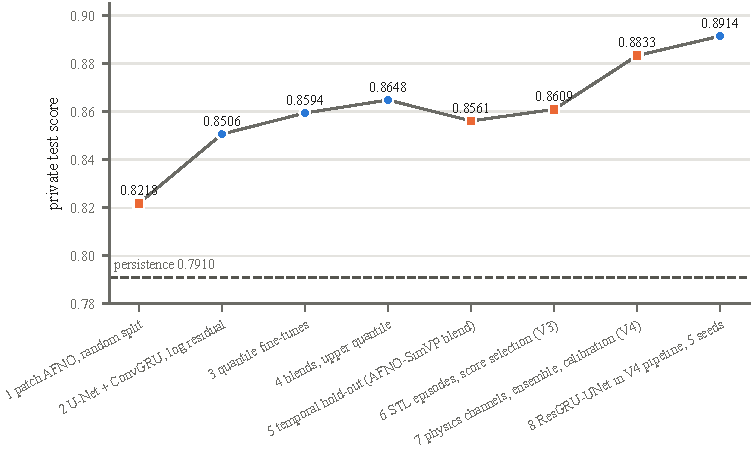
\includegraphics[width=\textwidth]{fig_pipeline_evolution.pdf}
\caption{Held-out test score at each development iteration. The dashed line is persistence (0.7910). Iteration 5 rebuilt the pipeline on an honest split and scored below iteration 4; the rebuilt pipeline overtakes it from iteration 6.}
\label{fig:evolution}
\end{figure*}

\textbf{1 to 2: from patch AFNO to ResGRU-UNet.} The first models followed FourCastNet: AFNO on $4\times4$ patches, trained on a random split. They stalled below 0.83 on the test set. The team read this as the global spectral layers acting as low-pass filters that blurred sharp spikes, and moved to a U-Net with full-resolution skips for local detail, a ConvGRU, and an output added to the last observed hour. The score rose to 0.8506. Later checks showed that the stated reason was not the mechanism. The patch model's spectral step applied the same complex matrix at every frequency, so apart from its soft threshold it was almost linear and local; a bug also discarded the imaginary half of every filtered spectrum; and each $4\times4$ patch was rebuilt by one linear layer with no skips. Three things had changed at once (the persistence residual, the skips and a log-space loss), and persistence alone is already strong.

\textbf{2 to 4: shifting forecasts up.} The base ResGRU-UNet under-predicted peaks. The team attributed this to losses that pull forecasts toward the centre and fine-tuned it in steps: a loss 20 times larger on under-predicted episode cells, then a pinball loss at the 0.75 quantile \cite{koenker1978}, then blends with models trained at the 0.85 and 0.90 quantiles. The test score rose at every step, from 0.8506 to 0.8648. The stated reason was wrong, since SMAPE is symmetric in the log ratio (Section~\ref{sec:theory}), but the action was right for another one: episode cells are picked where the truth turned out high, so upward-shifted forecasts score better on the episode terms. Scaling forecasts by hand did not help. ``Physics multipliers'' that raised stagnant cells by 25\% and all other cells by 12\% lost 0.006, because the 98\% of background cells pay for the shift, and a geometric blend with an AFNO member lost 0.008. Grafting four physics channels onto trained weights failed with NaN values.

\textbf{4 to 5: an honest split.} The random split gave an episode correlation near 0.98 for models that scored about 0.86 on the test set: with overlapping windows, it puts near-copies of every validation window into training. Iteration 5 held out the last 15 to 20\% of each month and rebuilt the model as AFNO with a SimVP-style temporal translator \cite{gao2022simvp}. Its best test score, 0.8561, came from a blend with ResGRU-UNet and was below iteration 4. An honest split does not raise the score; it makes choices trustworthy. And choices were still made on the wrong target: a proxy episode mask that marked 0.30\% of validation cells against about 2\% for the official one, checkpoints chosen on the validation loss, and no gap between training and validation windows.

\textbf{5 to 6: validation equal to the metric (V3).} V3 rewrote the pipeline so that validation measures exactly what the test measures: the official robust STL episodes, the exact score for choosing checkpoints, a 12-hour gap, per-cell normalization, a lead-hour embedding and weight averaging. It also fixed a hidden mismatch: the ResGRU-UNet models had been trained with the true hour of day but given hours 0 to 9 for every test window. In V3, training keeps the true hour, while validation and test windows get the estimated hour of Section~\ref{sec:physics}, so validation sees the same hour noise as the test. As one model with no blend, V3 reached 0.8609. Its validation now exposed what no earlier pipeline could see: global SMAPE kept improving after epoch 4 while episode SMAPE got worse.

\textbf{6 to 7: physics and calibration (V4).} V4 kept V3's pipeline and added what that diagnosis asked for: the ventilation, advection, tendency and diurnal-anomaly channels of Section~\ref{sec:physics}, one AFNO block at $35\times31$ for a middle scale \cite{dang2025adaptfno}, lead-hour weights because errors grow with lead time, two seeds, and per-hour calibration fitted on the honest hold-out. Calibration did in one fitted step what iterations 3 and 4 had done by hand, and the physics channels that failed as a graft worked as inputs trained from the start. The test score rose by 0.0224 to 0.8833.

\textbf{7 to 8: one pipeline for every network.} V4 was the best model, but its pipeline had changed together with its network: split, masks, inputs, loss, hour handling and post-processing. The other networks had been trained in older, leakier pipelines, so their scores could not be compared with V4's, and the question ``which network is better?'' had no clean answer. We therefore moved every network into V4's pipeline. Each was ported unchanged except for its input width (20 channels); ConvLSTM and patch AFNO also received the residual output with a zero-initialized last layer, ConvLSTM lost its season input, and patch AFNO got its bug fix. Each port was checked against its original (Section~\ref{sec:arch}). Each round-one notebook first re-evaluated the original AFNO V4 checkpoint on its own validation set and would have stopped unless it reproduced the logged 0.9110; it did, to five decimals. The windows, masks, loss, recipe and seed are then the same for every network, so the network is the only difference. Table~\ref{tab:samepipe} shows what the pipeline alone did for the three networks whose original runs are known: each gained 0.025 to 0.031 on the test set.

\begin{table}[!t]
\centering
\caption{The same network in its own pipeline and in the V4 pipeline (held-out test; V4 pipeline: seed 42, no ensemble or calibration). Each gain bundles every pipeline change, and for patch AFNO also its bug fix}
\label{tab:samepipe}
\begin{tabular}{@{}lccc@{}}
\toprule
Network & Own pipeline & V4 pipeline & Gain \\
\midrule
ResGRU-UNet & 0.8506 & 0.8798 & +0.0292 \\
FMG-WACLU & 0.8465 & 0.8710 & +0.0245 \\
patch AFNO & 0.8218 & 0.8530 & +0.0312 \\
\bottomrule
\end{tabular}
\end{table}

\section{Controlled backbone study}
\label{sec:study}
The study fixes everything in Sections~\ref{sec:setup} to \ref{sec:training} and changes only the network. It ran in three stages: one seed for all five networks; the two finalists with two seeds and the full V4 recipe; then five seeds per finalist.

\textbf{Round one.} Table~\ref{tab:round1}. ResGRU-UNet leads, and validation and test order the five networks the same way, which supports the validation design. Under the rule, ResGRU-UNet is better than AFNO V4 (+0.0048 validation, +0.0036 test), FMG-WACLU ties with it, and patch AFNO and ConvLSTM are worse.

\begin{table}[!t]
\centering
\caption{Round one: seed 42, same pipeline, no ensemble or calibration}
\label{tab:round1}
\begin{tabular}{@{}lrcc@{}}
\toprule
Network & Params & Validation & Test \\
\midrule
ResGRU-UNet & 7.12M & \textbf{0.9158} & \textbf{0.8798} \\
AFNO V4 & 6.98M & 0.9110 & 0.8762 \\
FMG-WACLU & 3.45M & 0.9099 & 0.8710 \\
patch AFNO & 5.71M & 0.9031 & 0.8530 \\
ConvLSTM & 19.0M & 0.8945 & 0.8452 \\
\bottomrule
\end{tabular}
\end{table}

\textbf{Two and five seeds.} With two seeds, ensembles and calibration for both, ResGRU-UNet again leads: 0.9175 against 0.9131 on validation and 0.8898 against 0.8833 on test. Five seeds give Table~\ref{tab:fiveseed} and Fig.~\ref{fig:seeds}. The validation gap between the five-seed means is $+0.00479$, with a 95\% block-bootstrap interval of $[+0.00383, +0.00578]$ (blocks of 13 consecutive windows within each month, 2{,}000 resamples). Every ResGRU-UNet seed beats every AFNO V4 seed on validation and on test (25 of 25 pairs); its worst seed (0.8788 test) beats AFNO V4's best (0.8767).

\begin{table}[!t]
\centering
\caption{Five seeds per finalist. Calibration is fitted on validation}
\label{tab:fiveseed}
\setlength{\tabcolsep}{4pt}
\begin{tabular}{@{}lccc@{}}
\toprule
 & AFNO V4 & ResGRU-UNet & Gap \\
\midrule
Single seeds, val: mean & 0.91146 & 0.91630 & +0.00484 \\
\quad standard deviation & 0.00059 & 0.00104 & \\
5-seed mean, val & 0.91454 & 0.91933 & +0.00479 \\
\ + calibration (one month out) & 0.91492 & 0.92097 & +0.00605 \\
Single seeds, test: mean & 0.87540 & 0.87994 & +0.00454 \\
\quad standard deviation & 0.00130 & 0.00085 & \\
5-seed mean, test & 0.8793 & 0.8838 & +0.0045 \\
\ + calibration, test & 0.8848 & \textbf{0.8914} & +0.0066 \\
\bottomrule
\end{tabular}
\end{table}

\begin{figure}[!t]
\centering
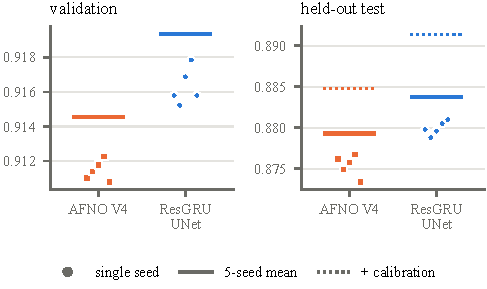
\includegraphics[width=\columnwidth]{fig_seed_spread.pdf}
\caption{Every seed of each finalist. The two families do not overlap on validation or on the held-out test.}
\label{fig:seeds}
\end{figure}

\textbf{Pipeline against backbone.} Moving ResGRU-UNet from iteration 2 into the V4 pipeline raised its test score from 0.8506 to 0.8798 (+0.0292, one seed, no calibration). At the same setting the gap to AFNO V4 is +0.0036, or +0.0045 averaged over five seeds. The pipeline therefore moved the score 6 to 8 times more than the choice between the two best networks (4.4 times against the full-recipe gap of +0.0066). The pipeline gain bundles several changes that we did not separate.

\section{Results}
\label{sec:results}
\subsection{Regression metrics}
Table~\ref{tab:regression} gives MAE, RMSE, $R^2$ and skill on validation for every model. The ridge baseline is one linear model shared by all cells: from the 20 channels at the last hour and $\log(1+y)$ at the nine earlier hours (30 features with a bias), it predicts the 16 log changes, fitted in closed form on 2.45 million training cell-windows (every fourth cell in each direction) with the penalty chosen on validation. With zero weights it is persistence. Every network beats all three baselines on every metric. The ResGRU-UNet ensemble has 31.8\% lower RMSE and 39.4\% lower MAE than persistence. Ridge improves on persistence on validation (score 0.8637) but barely on the test set (0.7951 against 0.7910).

\begin{table}[!t]
\centering
\caption{Validation regression metrics (MAE, RMSE in \ugm) over all $5.9\times10^7$ values, with the benchmark score $S$. Skill: lower RMSE than persistence. The hybrid row is out of fold (one month left out)}
\label{tab:regression}
\setlength{\tabcolsep}{2.6pt}
\begin{tabular}{@{}lrrrrr@{}}
\toprule
Model & MAE & RMSE & $R^2$ & Skill & $S$ \\
\midrule
Persistence & 10.44 & 26.46 & 0.767 & 0.0\% & 0.8515 \\
Seasonal naive (24 h) & 11.53 & 26.80 & 0.761 & $-1.3$\% & 0.7907 \\
Ridge regression & 8.51 & 21.48 & 0.847 & 18.8\% & 0.8637 \\
\midrule
\multicolumn{6}{@{}l}{\textit{Round one, seed 42}} \\
patch AFNO & 6.85 & 19.02 & 0.880 & 28.1\% & 0.9031 \\
ConvLSTM & 7.05 & 18.93 & 0.881 & 28.5\% & 0.8945 \\
FMG-WACLU & 7.14 & 19.32 & 0.876 & 27.0\% & 0.9099 \\
AFNO V4 & 7.31 & 20.17 & 0.865 & 23.8\% & 0.9110 \\
ResGRU-UNet & 6.57 & 18.57 & 0.885 & 29.8\% & 0.9158 \\
\midrule
\multicolumn{6}{@{}l}{\textit{Five-seed means}} \\
AFNO V4 & 6.99 & 19.45 & 0.874 & 26.5\% & 0.9145 \\
\ + calibration & 7.76 & 20.90 & 0.855 & 21.0\% & 0.9149 \\
ResGRU-UNet & \textbf{6.32} & 18.04 & 0.892 & 31.8\% & 0.9193 \\
\ + calibration & 7.12 & 19.71 & 0.871 & 25.5\% & \textbf{0.9210} \\
\ + LightGBM (hybrid) & 6.42 & \textbf{17.75} & \textbf{0.895} & \textbf{32.9\%} & 0.9051 \\
\bottomrule
\end{tabular}
\end{table}

\begin{figure*}[!t]
\centering
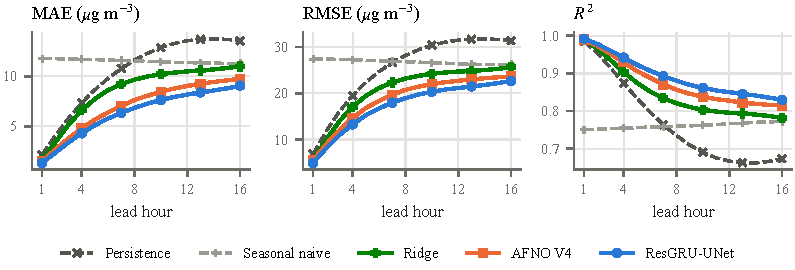
\includegraphics[width=\textwidth]{fig_lead_metrics.pdf}
\caption{Validation MAE, RMSE and $R^2$ by lead hour (five-seed means, no calibration). ResGRU-UNet is best at every hour. Seasonal naive overtakes persistence from hour 8, when the daily cycle outweighs the last observed state.}
\label{fig:lead}
\end{figure*}

\subsection{By lead hour and metric term}
Fig.~\ref{fig:lead} shows the error growing with lead time: ResGRU-UNet's $R^2$ falls from 0.992 at hour 1 to 0.830 at hour 16, and persistence's from 0.985 to 0.674. Fig.~\ref{fig:terms} splits the score into its three terms. ResGRU-UNet is better on all three at every hour; the score gap grows from $+0.0018$ at hour 1 to about $+0.006$ at hours 10 to 15. Of the five-seed gap, 56\% comes from global SMAPE, 23\% from episode SMAPE and 22\% from episode correlation.

\begin{figure*}[!t]
\centering
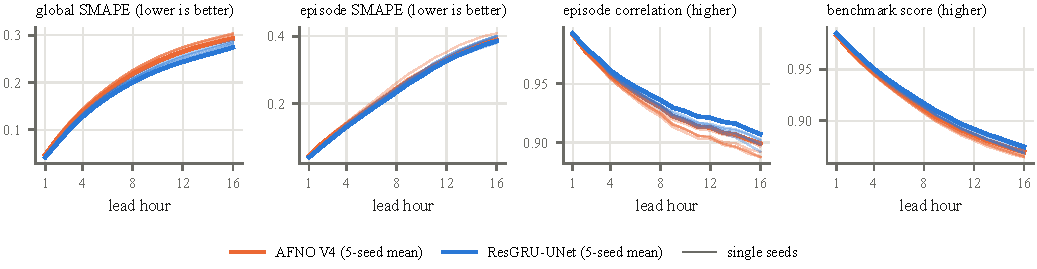
\includegraphics[width=\textwidth]{fig_terms_by_hour.pdf}
\caption{The three terms of the benchmark score and the score itself by lead hour, on validation. Thin lines: single seeds; thick lines: five-seed means.}
\label{fig:terms}
\end{figure*}

\subsection{Rankings depend on the metric}
ResGRU-UNet is first on all six measures in Fig.~\ref{fig:rank}, but the other four reorder. AFNO V4 is second on the benchmark score yet last on MAE, RMSE and $R^2$; ConvLSTM is last on the score yet second on RMSE and $R^2$. The score is relative and focused on episodes, while raw-scale MAE, RMSE and $R^2$ are dominated by high concentrations. One metric alone would have misjudged the weaker networks.

\begin{figure}[!t]
\centering
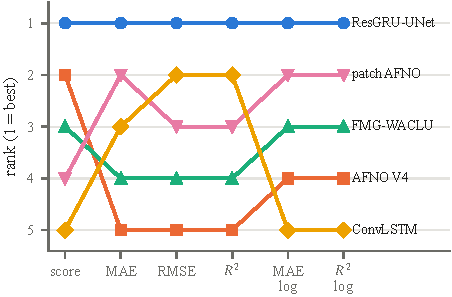
\includegraphics[width=\columnwidth]{fig_rank_by_metric.pdf}
\caption{Round-one ranks (seed 42) under six measures. Only the winner is stable.}
\label{fig:rank}
\end{figure}

\subsection{Calibration trades error for score}
Calibration raises the score but worsens MAE, RMSE and $R^2$ for both finalists (Fig.~\ref{fig:calib}): the ResGRU-UNet ensemble moves from MAE 6.32 to 7.12 while its score rises from 0.9193 to 0.9210. The factors push forecasts up, which the episode terms reward and absolute and squared errors penalize. The uncalibrated mean is the better model for MAE, RMSE and $R^2$; the calibrated one is better for the benchmark score.

\begin{figure}[!t]
\centering
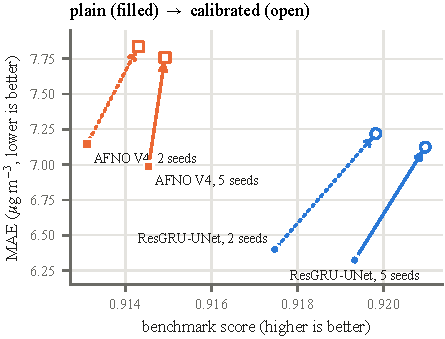
\includegraphics[width=\columnwidth]{fig_calibration.pdf}
\caption{Calibration moves both finalists to a higher score and a higher MAE (validation; in sample for 2 seeds, leave one month out for 5 seeds).}
\label{fig:calib}
\end{figure}

\subsection{ML + DL hybrid: a boosted correction}
\label{sec:hybrid}
We tested whether a classical model can correct the network. A LightGBM model \cite{ke2017lightgbm} (300 trees, 31 leaves, Huber loss, fixed settings) predicts the error of the uncalibrated ResGRU-UNet five-seed ensemble in $\log(1+y)$, and the forecast is shifted by it. It uses 33 features per cell and lead hour: the 20 input channels at the last hour, $\log(1+y)$ at the nine earlier hours, the ensemble forecast, its change from the last hour, the spread of the five seeds, and the lead hour. It is fitted on every fourth cell in each direction. The rule was written before the run: fit on the validation windows of three months and predict the fourth, for all four months, and call the hybrid better only if its pooled score is higher and it wins in at least three months.

The verdict is no gain. The hybrid scores lower in all four held-out months ($-0.0162$, $-0.0151$, $-0.0068$ and $-0.0188$ for April, July, October and December) and 0.9051 against 0.9193 pooled. RMSE and $R^2$ improve slightly (17.75 against 18.04; 0.895 against 0.892) and MAE is slightly worse (6.42 against 6.32), but episode SMAPE rises from 0.235 to 0.305. This is the calibration trade-off in reverse, and it fits the theory of Section~\ref{sec:theory}: a symmetric loss in log space pulls forecasts toward the typical value, which removes the upward shift that the episode terms reward. The model leaned most on the forecast's change from the last hour and on the seed spread (15\% and 13\% of its split gain). The hybrid was not submitted to the test set, as the rule required a win first.

\subsection{Where ResGRU-UNet wins}
It is ahead in all four validation months and in five of six concentration bins (Fig.~\ref{fig:where}). Both models under-predict episode cells (mean log bias $-0.160$ for AFNO V4 and $-0.157$ for ResGRU-UNet) and over-predict the other cells ($+0.084$ and $+0.062$), most of all in the cleanest bin (Fig.~\ref{fig:where}, middle). ResGRU-UNet's smaller over-prediction outside episodes is consistent with its larger gain in the global term.

\begin{figure*}[!t]
\centering
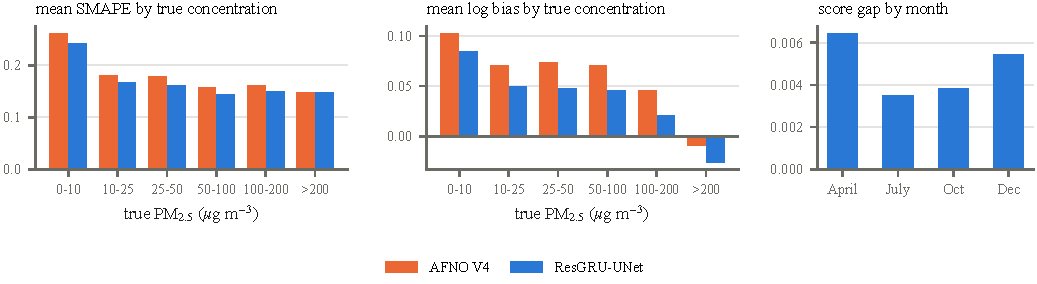
\includegraphics[width=\textwidth]{fig_where.pdf}
\caption{Five-seed means on validation. Left: mean SMAPE by true concentration. Middle: mean log bias (positive: too high). Right: score gap by month (ResGRU-UNet minus AFNO V4).}
\label{fig:where}
\end{figure*}

\subsection{Spatial structure}
Fig.~\ref{fig:maps} maps the time-averaged errors. \PM{} and the errors of persistence concentrate over the Indo-Gangetic Plain and the eastern coal belt; ResGRU-UNet removes much of that error. It has lower MAE than AFNO V4 in 90.5\% of cells and lower SMAPE in 94.7\% (Fig.~\ref{fig:smape}), with the largest gains over the Indo-Gangetic Plain and central India. The median per-cell $R^2$ over time is 0.872 for ResGRU-UNet, 0.846 for AFNO V4 and 0.694 for persistence; it is lowest north of 32$^\circ$N (median 0.764), where the air is cleanest (13.8 against 42.3~\ugm{} south of it). Fig.~\ref{fig:case} shows the window with the most episode cells.

\begin{figure*}[!t]
\centering
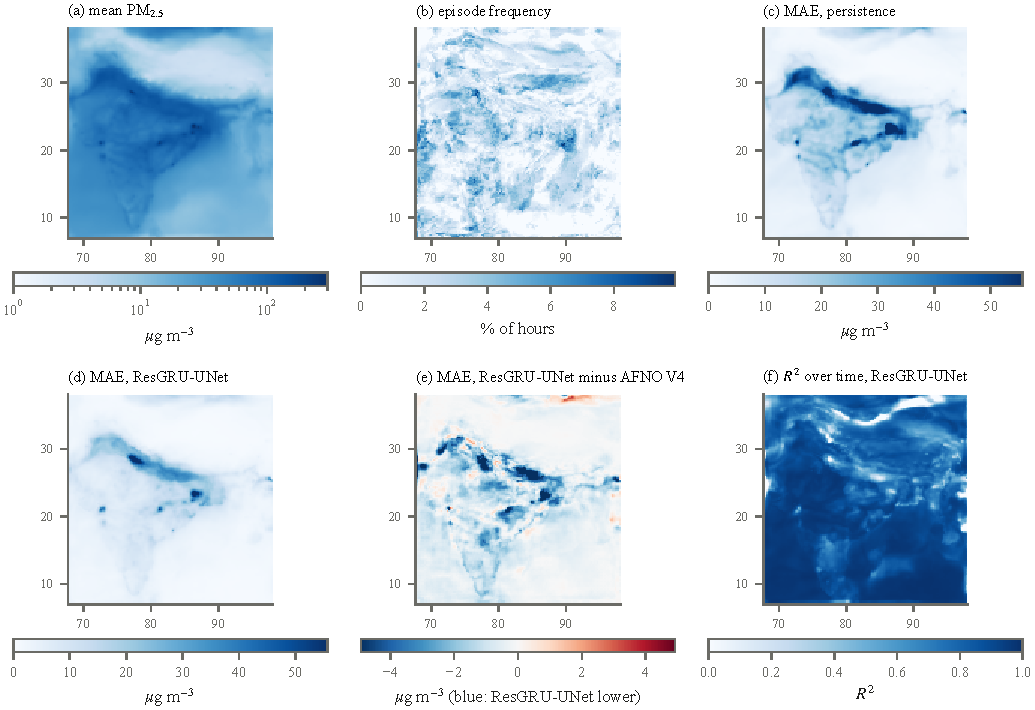
\includegraphics[width=\textwidth]{fig_maps.pdf}
\caption{Time-averaged validation maps. (a) Mean \PM. (b) Share of hours that are episodes. (c, d) MAE of persistence and of the ResGRU-UNet five-seed mean. (e) MAE difference, ResGRU-UNet minus AFNO V4. (f) $R^2$ of each cell's time series, ResGRU-UNet.}
\label{fig:maps}
\end{figure*}

\begin{figure*}[!t]
\centering
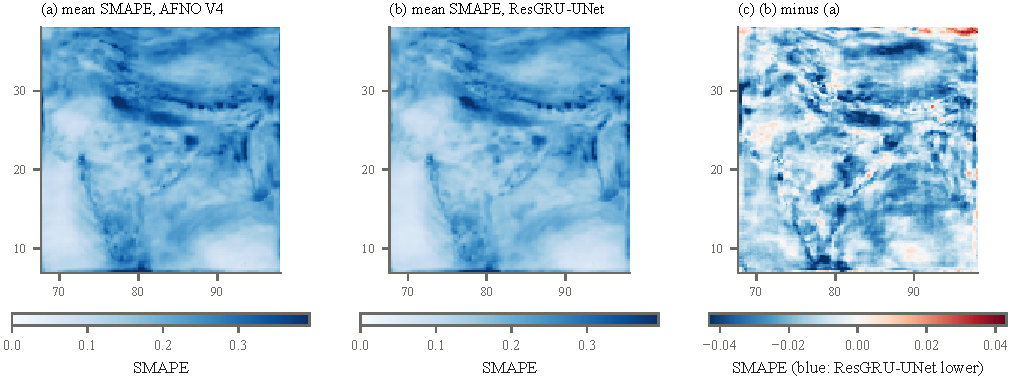
\includegraphics[width=\textwidth]{fig_smape_maps.pdf}
\caption{Mean SMAPE per cell for the five-seed means of AFNO V4 (a) and ResGRU-UNet (b), and their difference (c). ResGRU-UNet is lower in 94.7\% of cells.}
\label{fig:smape}
\end{figure*}

\begin{figure}[!t]
\centering
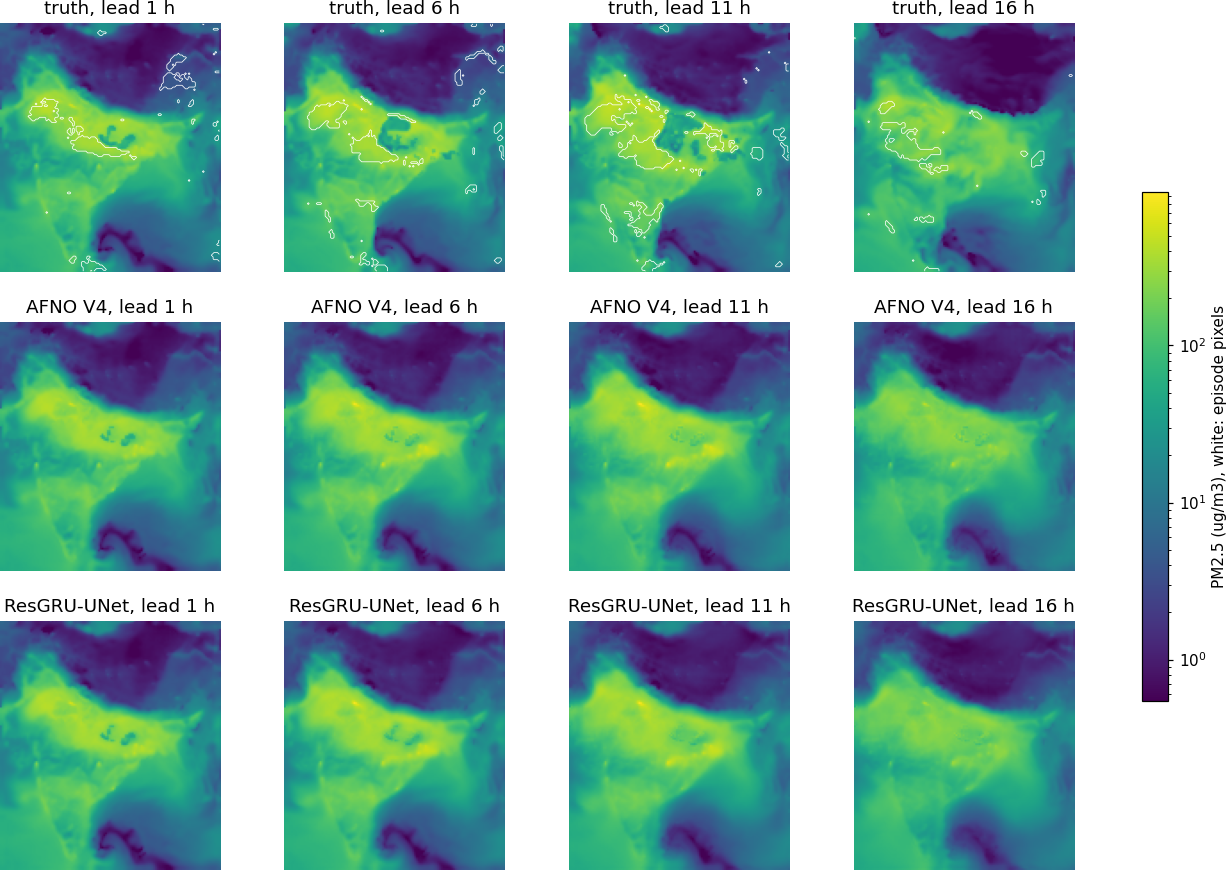
\includegraphics[width=\columnwidth, trim=155 79 194 71, clip]{fig_case.png}
\caption{The validation window with the most episode cells (December): truth with episode cells outlined (top), AFNO V4 (middle) and ResGRU-UNet (bottom) at lead hours 1, 6, 11 and 16, in grid coordinates on a log colour scale. Both smooth the episode structure; ResGRU-UNet scores higher on this window (0.9116 against 0.9103) but has the lower episode correlation (0.928 against 0.944).}
\label{fig:case}
\end{figure}

\subsection{Cost}
ResGRU-UNet is also cheaper: 25.8 against 48.6~ms per window at inference, 0.23 against 1.36~GB of peak inference memory at batch 4, and 191 against 338~s per training epoch on a T4.

\section{Ablation studies}
\label{sec:ablation}
\textbf{What V4's pipeline steps added.} V4's test gain over V3 (+0.0224) splits into +0.0147 from the per-seed changes (physics channels, multiscale block, horizon weights), +0.0024 from the two-seed ensemble and +0.0054 from calibration (65\%, 10\% and 24\%), measured by submitting the intermediate forecasts.

\textbf{Why the convolutional-recurrent network wins.} We tested four hypotheses, each with one change to one finalist and one seed (Table~\ref{tab:ablations}), with predictions written down first. A change counts only if it moves validation by more than $\max(2\,\mathrm{sd}, 0.002)$ from its family's five-seed mean:
\begin{itemize}
\item H1: AFNO V4's skips keep only the last hour and the mean;
\item H2: the FFT wraps opposite edges of a non-periodic map;
\item H3: the soft threshold removes small details;
\item H4: ResGRU-UNet wins because of its recurrence over lead time.
\end{itemize}
None passes the threshold at one seed. H1 (skips that fuse all 10 hours, started equal to V4's fusion) moves AFNO V4 about a quarter of the way toward ResGRU-UNet. Replacing ResGRU-UNet's ConvGRU with per-lead convolution blocks of the same size costs about a third of the gap, yet it still beats every AFNO V4 seed: the recurrence is not needed to win, but its share is unresolved. Padding also strengthens the soft threshold, because the orthonormal FFT spreads the same energy over four times as many coefficients; H3 suggests this matters little.

\begin{table}[!t]
\centering
\caption{Single-change ablations (seed 42). $d$: validation change from the family's five-seed mean; $d/G$: share of the 0.00484 gap. Threshold 0.002}
\label{tab:ablations}
\setlength{\tabcolsep}{3pt}
\begin{tabular}{@{}lp{0.4\columnwidth}rrr@{}}
\toprule
 & Change & $d$ & $d/G$ & Test \\
\midrule
H1 & AFNO V4, skips fuse all 10 hours & $+0.00113$ & $+0.23$ & 0.8748 \\
H2 & AFNO V4, zero-padded FFT & $-0.00084$ & $-0.17$ & 0.8745 \\
H3 & AFNO V4, no soft threshold & $-0.00052$ & $-0.11$ & 0.8758 \\
H4 & ResGRU-UNet, ConvGRU replaced & $-0.00174$ & $-0.36$ & 0.8798 \\
\bottomrule
\end{tabular}
\end{table}

\textbf{A generalization gap.} The training curves (Fig.~\ref{fig:curves}) show a pattern none of the AFNO changes altered. Every AFNO run reaches a lower training loss than ResGRU-UNet but a higher validation loss: at a training loss of 0.09, its validation loss is 6.8\% higher on average. Its score peaks at epoch 4 or 5 and then falls by 0.009 to 0.010; ResGRU-UNet peaks at epoch 6 or 7 and falls by 0.003 to 0.005. Without its recurrence, ResGRU-UNet moves about 41\% of the way toward AFNO's validation loss. These observations are exploratory, but they suggest AFNO V4 fits the training months more and transfers less to new months. Its global, wrap-around spectral mixing, per-hour encoder and translator remain candidates for the cause.

\begin{figure}[!t]
\centering
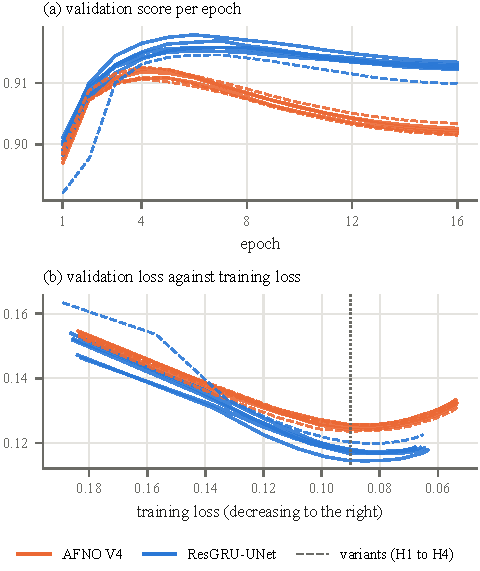
\includegraphics[width=\columnwidth]{fig_training_curves.pdf}
\caption{Training curves of the 12 logged runs: (a) validation score per epoch; (b) validation loss against training loss, with a dotted line at a training loss of 0.09.}
\label{fig:curves}
\end{figure}

\section{Limitations}
\begin{itemize}
\item The data are simulations, not measurements, and skill on WRF-Chem fields need not carry over to monitored \PM.
\item There is one validation period and one test set. Validation picked each run's best epoch and fitted the calibration, so validation scores are optimistic; the test set is the only untouched measure, and it reports only the benchmark score.
\item The score's weights are not disclosed; we assume equal weights on validation.
\item The recipe was tuned for AFNO V4, which if anything favours it; ResGRU-UNet was not tuned.
\item The later rounds were designed after round one's result, adjacent bootstrap blocks overlap in time, and the ablations use one seed each.
\item The pipeline gain bundles several changes that we did not separate.
\item The hybrid was tested in one fixed configuration, on the validation windows that also chose each network's best epoch, and has no test score.
\end{itemize}

\section{Conclusion}
For 16-hour \PM{} forecasting over India, the pipeline mattered more than the network. Physics channels for mixing and transport, a log-space persistence residual, validation that reproduces the test, a loss matched to the score, and ensembling with calibration gave the same network a gain 6 to 8 times the gap between the two best networks. Inside one fixed pipeline, a plain convolutional-recurrent U-Net beat the Fourier neural operator hybrid on every seed pair, lead hour, month and regression metric, and it is also cheaper to run. No single component we tested explains the gap; the Fourier model generalizes less well across months, which fits a transport problem that is local and not periodic. A gradient-boosted correction of the ensemble lowered squared error but not the benchmark score, so the next step for a hybrid is a correction trained on the score's own terms, as the networks are.

\section*{Reproducibility}
The code is at \url{https://github.com/Vetri-78640/dl_pm2.5}: the shared pipeline and every network (\texttt{src/}), the notebook builders and Kaggle tools (\texttt{scripts/}), the dry runs, port check and config test (\texttt{tests/}), six local notebooks with outputs (\texttt{notebooks/}; \texttt{notebooks/kaggle/} holds the Kaggle notebooks exactly as they ran, with their run logs), the study settings (\texttt{configs/}), the run records (\texttt{results/}), the AFNO V4 script and the original notebooks of the ported networks (\texttt{reference/}), and the result tables, figures and this report (\texttt{reports/}). The competition data is not included; see \texttt{data/README.md}.

\section*{Team contributions}
\begin{itemize}
\item \textbf{Ishan Goyal}: data and pre-processing: data analysis, the 20 input channels, normalization, the hour estimate, the leak-free split and episode masks.
\item \textbf{Vetriselvan R}: study design and decision rules (fixed before training); model architectures: AFNO V4, ResGRU-UNet, the ports of the other three networks, the port check and the ablation variants; the round-one, final-round, ablation and hybrid runs; and this report.
\item \textbf{Hrishi Dongre}: training pipeline: loss, optimizer and schedule, weight averaging, checkpoints and resume, the notebook builders and the seed runs.
\item \textbf{Vedant Madne}: evaluation and post-processing: seed ensembles and calibration, the persistence, seasonal-naive and ridge baselines, and MAE, RMSE and $R^2$.
\item \textbf{Pampana Sree Adithya}: experiments and analysis: 5-seed statistics and block bootstrap, the ablation verdict, figures and error maps.
\end{itemize}

\begin{thebibliography}{99}
\bibitem{phase1} Vetriselvan R, H. Dongre, P. S. Adithya, I. Goyal, and V. Madne, ``Six-hour PM2.5 forecasting in Beijing with gradient boosting and leak-free testing,'' Team T024 Phase 1 project report, 2026.
\bibitem{aisehack2026} ANRF AISEHack 2026, Phase 2, Theme 2: pollution forecasting (IIT Delhi), Kaggle, 2026. [Online]. Available: \url{https://www.kaggle.com/competitions/anrf-aise-hack-phase-2-theme-2-pollution-forecasting-iitd}
\bibitem{pandey2021} A. Pandey \emph{et al.}, ``Health and economic impact of air pollution in the states of India: The Global Burden of Disease Study 2019,'' \emph{Lancet Planet. Health}, vol. 5, no. 1, pp. e25--e38, 2021.
\bibitem{grell2005} G. A. Grell, S. E. Peckham, R. Schmitz, S. A. McKeen, G. Frost, W. C. Skamarock, and B. Eder, ``Fully coupled `online' chemistry within the WRF model,'' \emph{Atmos. Environ.}, vol. 39, no. 37, pp. 6957--6975, 2005.
\bibitem{kushwaha2025} A. Kushwaha and K. Gopalan, ``A comparison of lightweight deep learning models for particulate-matter nowcasting in the Indian subcontinent \& surrounding regions,'' arXiv:2511.11185, 2025.
\bibitem{bedi2025conoair} S. Bedi, K. Tiwari, Prathosh A. P., S. H. Kota, N. M. A. Krishnan \emph{et al.}, ``CoNOAir: A neural operator for forecasting carbon monoxide evolution in cities,'' arXiv:2501.06007, 2025.
\bibitem{li2021fno} Z. Li, N. Kovachki, K. Azizzadenesheli, B. Liu, K. Bhattacharya, A. Stuart, and A. Anandkumar, ``Fourier neural operator for parametric partial differential equations,'' in \emph{Proc. ICLR}, 2021.
\bibitem{guibas2022afno} J. Guibas, M. Mardani, Z. Li, A. Tao, A. Anandkumar, and B. Catanzaro, ``Efficient token mixing for transformers via adaptive Fourier neural operators,'' in \emph{Proc. ICLR}, 2022.
\bibitem{pathak2022fourcastnet} J. Pathak \emph{et al.}, ``FourCastNet: A global data-driven high-resolution weather model using adaptive Fourier neural operators,'' arXiv:2202.11214, 2022.
\bibitem{dang2025adaptfno} H. V. Dang, B. D. G. Nguyen, P. C. H. Nguyen, and T.-S. Hy, ``AdaptFNO: Adaptive Fourier neural operator with dynamic spectral modes and multiscale learning for climate modeling,'' in \emph{NeurIPS Workshop on Machine Learning and the Physical Sciences}, 2025.
\bibitem{shi2015convlstm} X. Shi, Z. Chen, H. Wang, D.-Y. Yeung, W.-k. Wong, and W.-c. Woo, ``Convolutional LSTM network: A machine learning approach for precipitation nowcasting,'' in \emph{Proc. NeurIPS}, 2015, pp. 802--810.
\bibitem{shi2017trajgru} X. Shi, Z. Gao, L. Lausen, H. Wang, D.-Y. Yeung, W.-k. Wong, and W.-c. Woo, ``Deep learning for precipitation nowcasting: A benchmark and a new model,'' in \emph{Proc. NeurIPS}, 2017.
\bibitem{ballas2016convgru} N. Ballas, L. Yao, C. Pal, and A. Courville, ``Delving deeper into convolutional networks for learning video representations,'' in \emph{Proc. ICLR}, 2016.
\bibitem{ronneberger2015unet} O. Ronneberger, P. Fischer, and T. Brox, ``U-Net: Convolutional networks for biomedical image segmentation,'' in \emph{Proc. MICCAI}, 2015, pp. 234--241.
\bibitem{he2016} K. He, X. Zhang, S. Ren, and J. Sun, ``Deep residual learning for image recognition,'' in \emph{Proc. CVPR}, 2016, pp. 770--778.
\bibitem{gao2022simvp} Z. Gao, C. Tan, L. Wu, and S. Z. Li, ``SimVP: Simpler yet better video prediction,'' in \emph{Proc. CVPR}, 2022, pp. 3170--3180.
\bibitem{leinonen2021} J. Leinonen, ``Spatiotemporal weather data predictions with shortcut recurrent-convolutional networks: A solution for the Weather4cast challenge,'' arXiv:2111.02121, 2021.
\bibitem{loshchilov2019} I. Loshchilov and F. Hutter, ``Decoupled weight decay regularization,'' in \emph{Proc. ICLR}, 2019.
\bibitem{smith2019} L. N. Smith and N. Topin, ``Super-convergence: Very fast training of neural networks using large learning rates,'' in \emph{Proc. SPIE}, vol. 11006, 2019.
\bibitem{wu2018} Y. Wu and K. He, ``Group normalization,'' in \emph{Proc. ECCV}, 2018, pp. 3--19.
\bibitem{polyak1992} B. T. Polyak and A. B. Juditsky, ``Acceleration of stochastic approximation by averaging,'' \emph{SIAM J. Control Optim.}, vol. 30, no. 4, pp. 838--855, 1992.
\bibitem{lakshminarayanan2017} B. Lakshminarayanan, A. Pritzel, and C. Blundell, ``Simple and scalable predictive uncertainty estimation using deep ensembles,'' in \emph{Proc. NeurIPS}, 2017, pp. 6402--6413.
\bibitem{goodwin1999} P. Goodwin and R. Lawton, ``On the asymmetry of the symmetric MAPE,'' \emph{Int. J. Forecast.}, vol. 15, no. 4, pp. 405--408, 1999.
\bibitem{roberts2017} D. R. Roberts \emph{et al.}, ``Cross-validation strategies for data with temporal, spatial, hierarchical, or phylogenetic structure,'' \emph{Ecography}, vol. 40, no. 8, pp. 913--929, 2017.
\bibitem{kaufman2012} S. Kaufman, S. Rosset, C. Perlich, and O. Stitelman, ``Leakage in data mining: Formulation, detection, and avoidance,'' \emph{ACM Trans. Knowl. Discov. Data}, vol. 6, no. 4, Art. no. 15, 2012.
\bibitem{hyndman2021} R. J. Hyndman and G. Athanasopoulos, \emph{Forecasting: Principles and Practice}, 3rd ed. Melbourne, Australia: OTexts, 2021.
\bibitem{hoerl1970} A. E. Hoerl and R. W. Kennard, ``Ridge regression: Biased estimation for nonorthogonal problems,'' \emph{Technometrics}, vol. 12, no. 1, pp. 55--67, 1970.
\bibitem{cleveland1990} R. B. Cleveland, W. S. Cleveland, J. E. McRae, and I. Terpenning, ``STL: A seasonal-trend decomposition procedure based on loess,'' \emph{J. Off. Stat.}, vol. 6, no. 1, pp. 3--73, 1990.
\bibitem{iyer2013} U. S. Iyer and P. E. Raj, ``Ventilation coefficient trends in the recent decades over four major Indian metropolitan cities,'' \emph{J. Earth Syst. Sci.}, vol. 122, no. 2, pp. 537--549, 2013.
\bibitem{staniforth1991} A. Staniforth and J. C\^{o}t\'{e}, ``Semi-Lagrangian integration schemes for atmospheric models: A review,'' \emph{Mon. Weather Rev.}, vol. 119, no. 9, pp. 2206--2223, 1991.
\bibitem{ke2017lightgbm} G. Ke \emph{et al.}, ``LightGBM: A highly efficient gradient boosting decision tree,'' in \emph{Adv. Neural Inf. Process. Syst.}, vol. 30, 2017, pp. 3146--3154.
\bibitem{koenker1978} R. Koenker and G. Bassett Jr., ``Regression quantiles,'' \emph{Econometrica}, vol. 46, no. 1, pp. 33--50, 1978.
\end{thebibliography}

\end{document}
